\section{Simulation Analysis}
\label{sec:simulation}

\subsection{Transient analysis}

We simulated the circuit using transient analysis, using the supplied model of transistors:

\begin{table}[H]
\addtolength{\tabcolsep}{-4pt}
\caption{Values of capacitances and resistances for various circuit components}
\vspace{-3mm}
\begin{tabular}{|c|c|c|}
\hline
Vc = 12.0 V
f=1e3 Hz
Vs = 10e-3 V
Rs = 100 $\Ohm$
Ci = 1e-3 $F$
Rb1 = 80e3 $\Ohm$
Rb2 =20e3 $\Ohm$
Rc = 1e3 $\Ohm$
Re =100 $\Ohm$
Ce = 1e-3 $F$
Von=0.7 V
Vt=25e-3 V
Va1=69.7 V
Va2=37.2 V
Rd = 100 $\Ohm$
Co = 1e-6 $F$
Rl = 8 $\Ohm$

\hline
\end{tabular}
\label{tab:Components}
\end{table}

\par

We simulate 

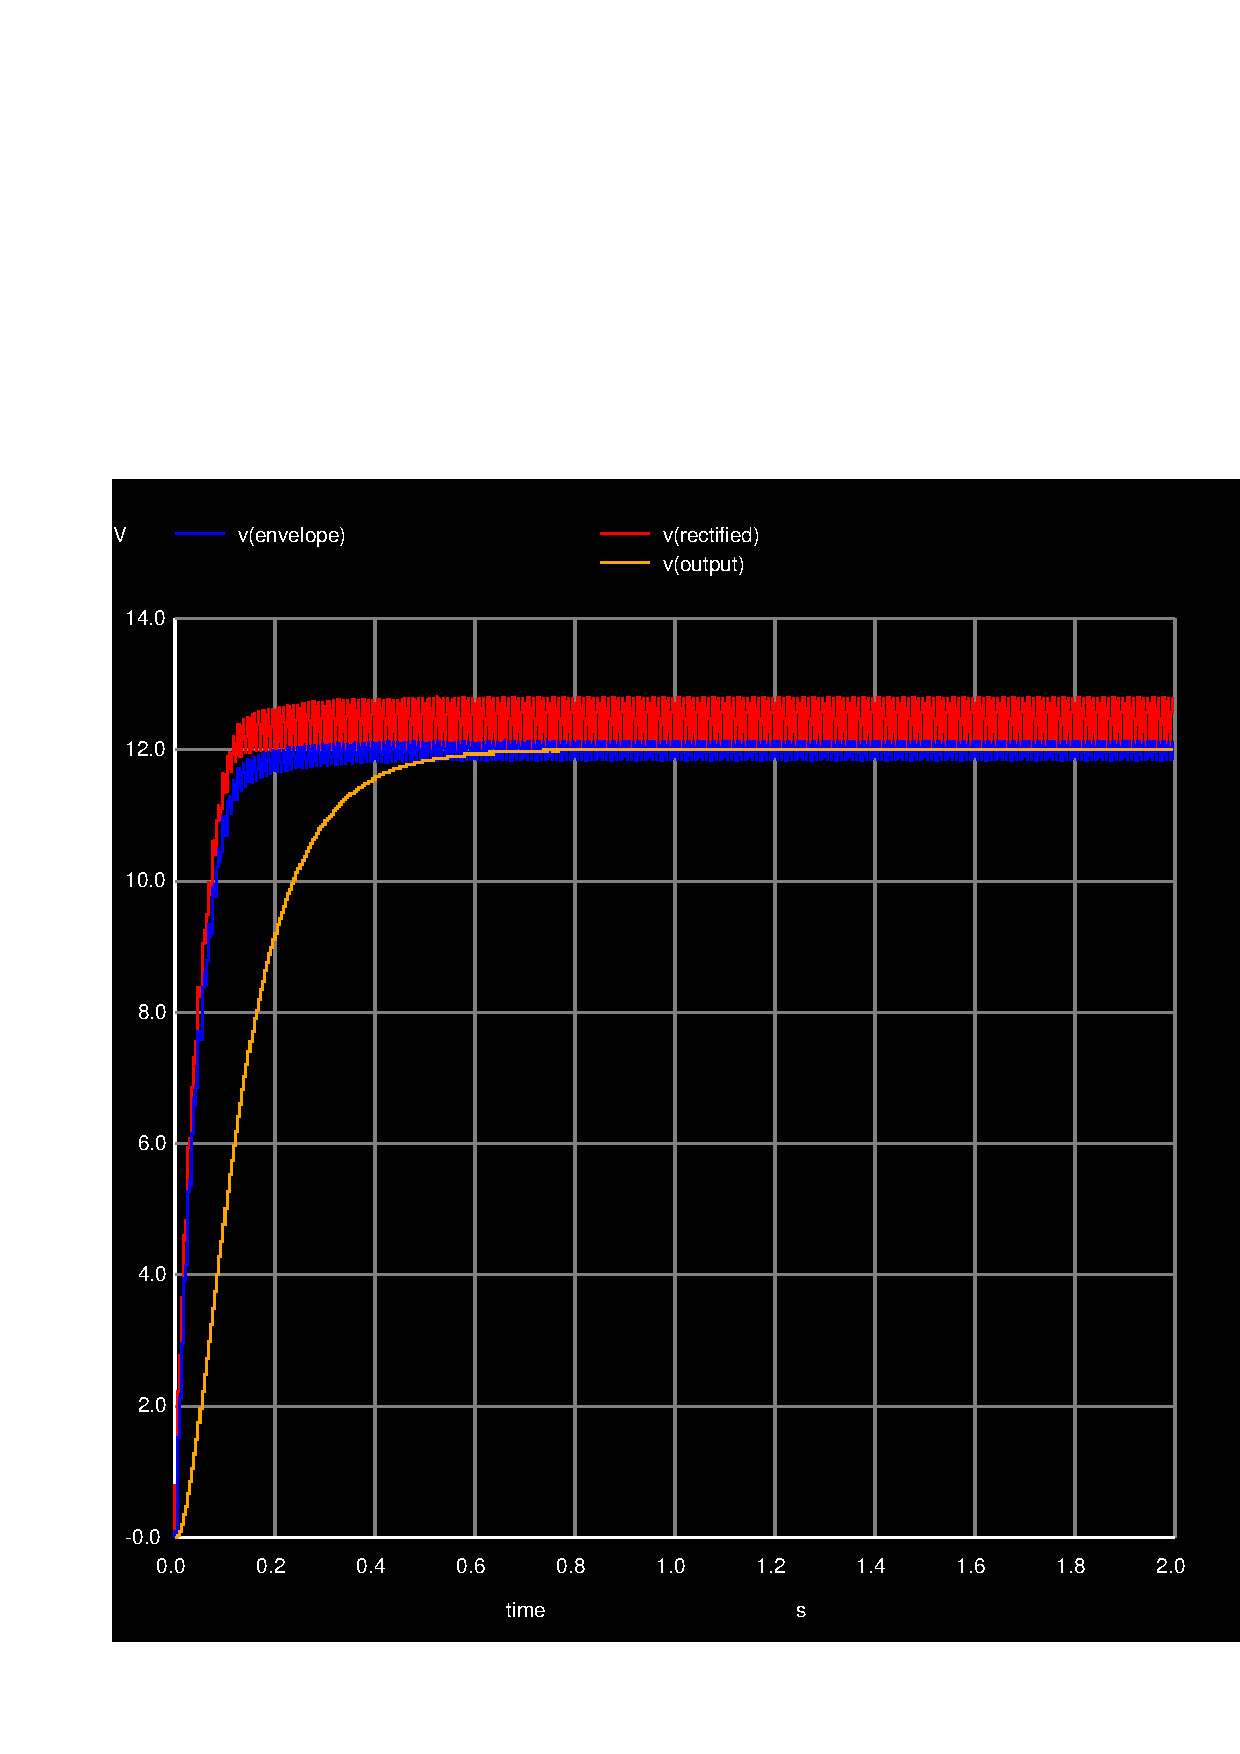
\includegraphics[width=1\linewidth]{../sim/vinit.pdf}

\par

By choosing a 10 period section in which the circuit has already stabelized, we can better study it.

\begin{minipage}[c]{0.50\linewidth}
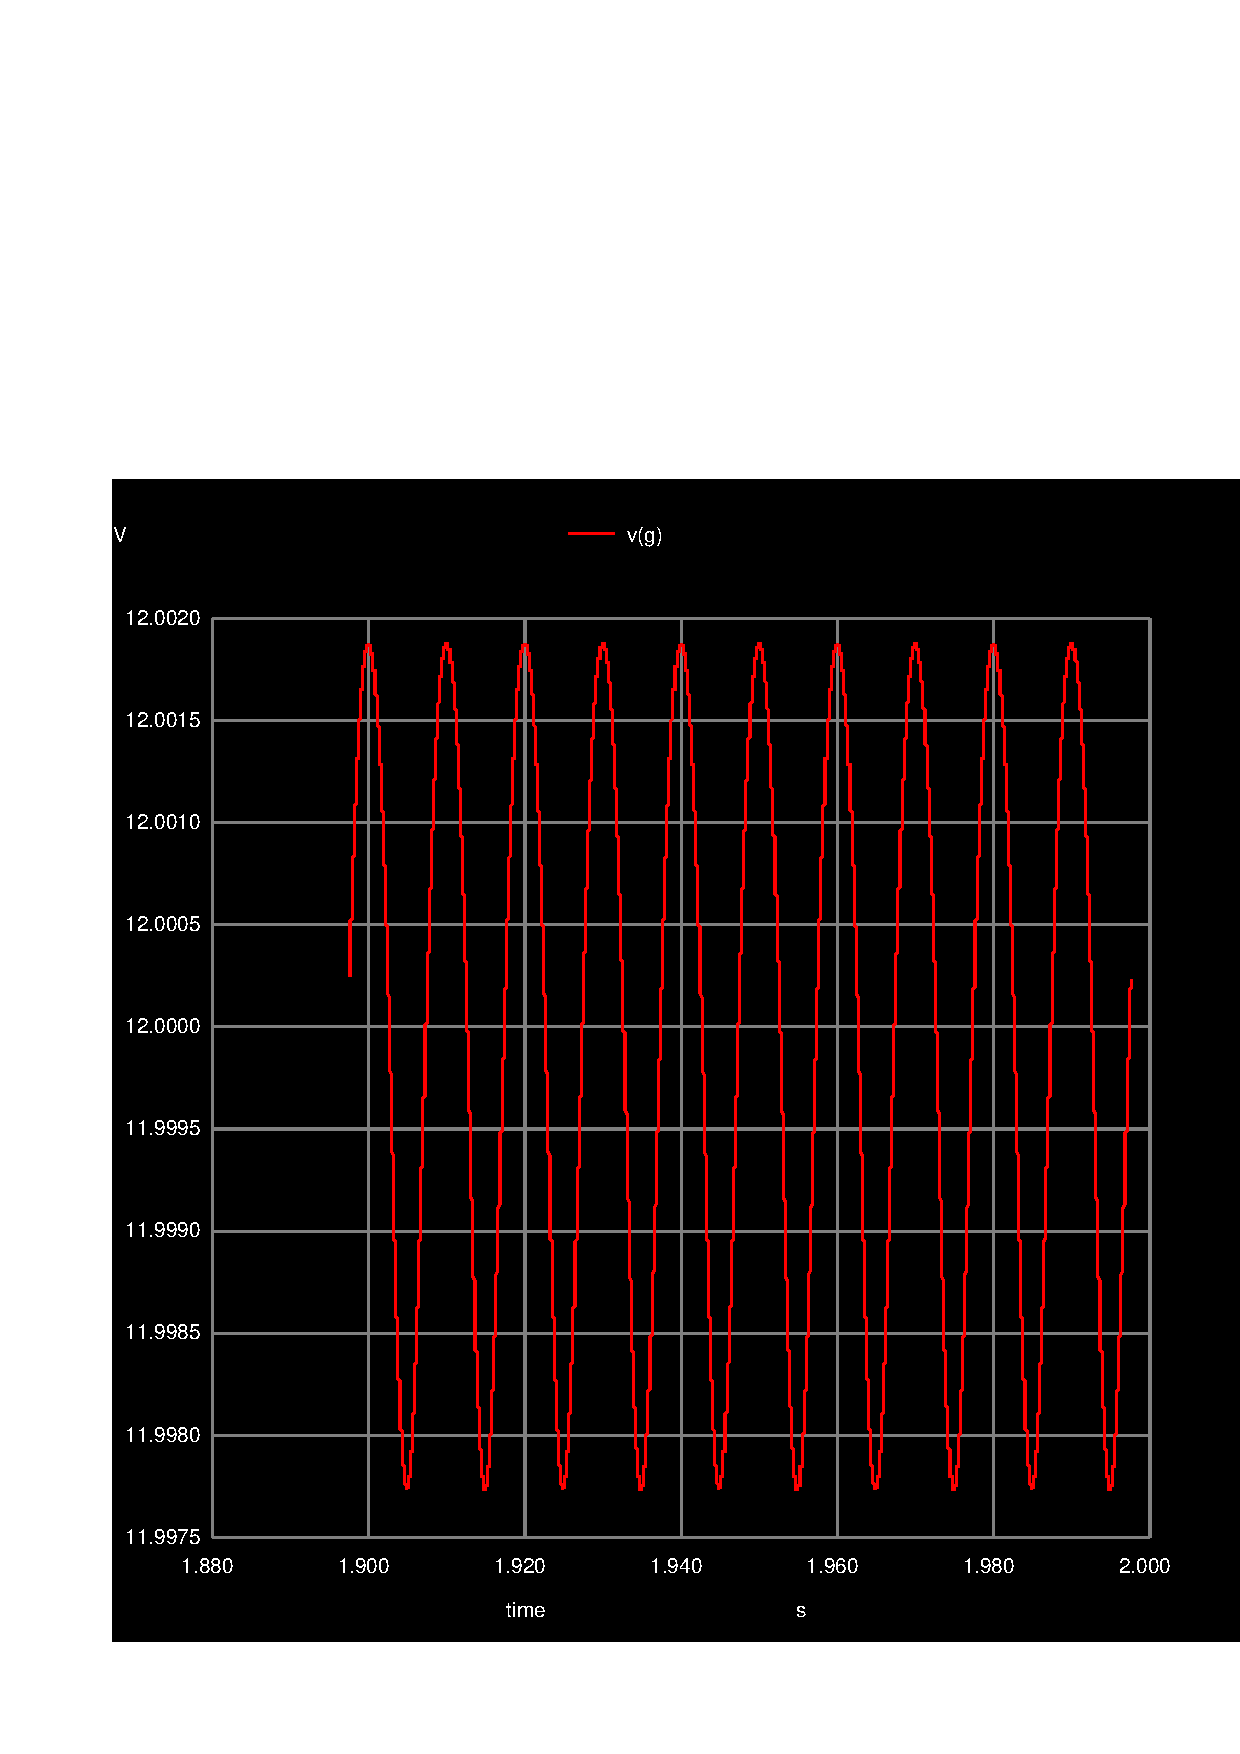
\includegraphics[width=1\linewidth]{../sim/vout.pdf}
\end{minipage} % no space if you would like to put them side by side
\hspace{1mm}
\begin{minipage}[c]{0.50\linewidth}
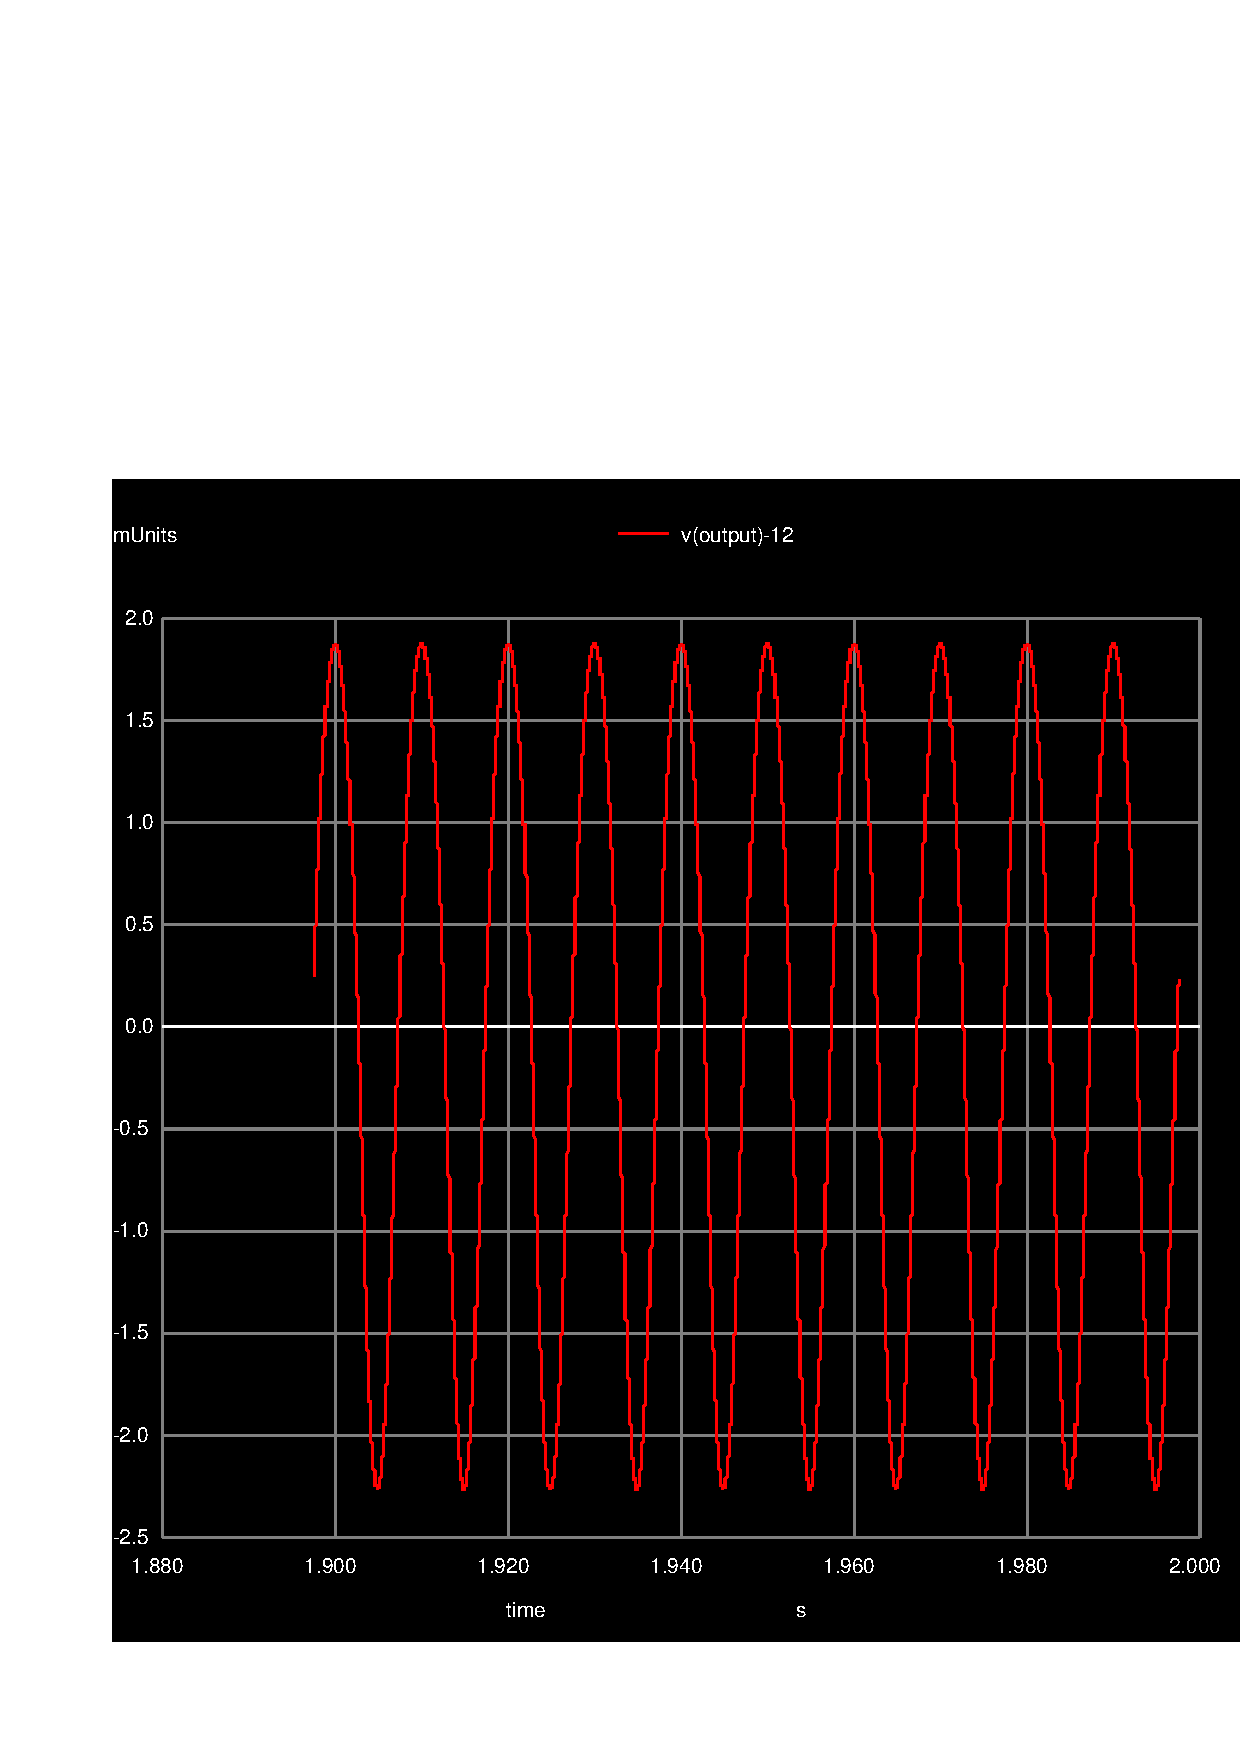
\includegraphics[width=1\linewidth]{../sim/v12.pdf}
\end{minipage}
    
The average of $V_{out}$ in equilibrium is 12.000000V and the ripple is 4.13 mV. The circuit costs 59.9448 monetary units, and the calculated merit is 4.038251.
